\vspace{-5pt} 
\subsection{One-dimensional Projection Algorithm}

In this section, a one-dimensional projection algorithm ({\sc 1DPA}) is presented. Efficient approximation algorithms for classical knapsack problem have been proposed in the literature \cite{KSbook}. However, the problems concerned in this paper belong to a two-dimensional generalization of the one-dimensional classical knapsack problem, for which the immediate application of these algorithms for knapsack problem cannot be applied. A plausible approach is to reduce the two-dimensional problems onto a one-dimensional instance by a proper projection of the power demand vectors to a certain reference vector.

First, consider {\sc maxPA}. The basic idea is to project all power demand vectors onto the $\frac{\pi}{4}$ line (see Fig.~\ref{fig:projection} for an illustration). Namely, create a new vector along the $\frac{\pi}{4}$ line with magnitude $\tilde{S}_k = \frac{P_k + Q_k}{\sqrt{2}}$ for each $S_k = P_k + {\bf i} Q_k$. Then apply the well-known efficient approximation algorithm for the classical knapsack problem \cite{KSbook} (denoted by ${\rm Alg}^{\rm kp}$) on the set $\{\tilde{S}_k\}_{k \in {\cal N}}$ and capacity $\frac{C}{\sqrt{2}}$. 
Lastly, return the maximum valuation of two candidate solutions: either the solution by ${\rm Alg}^{\rm kp}$, or the maximum valuation of a single customer $\arg\max_{k\in \cN} \{u_k\}$. Fig.~\ref{fig:alg0.5} presents a flowchart of {\sc 1DPA}.


\begin{figure}[!ht]
\centering \vspace{-5pt} 
 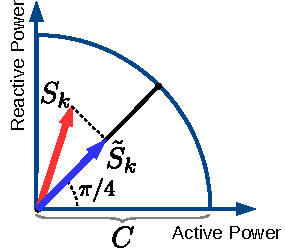
\includegraphics[scale=0.7]{{fig/fig-0.5-alg}.pdf} %\vspace{-5pt} 
 \caption{Each power demand $S_k$ is projected onto the $\frac{\pi}{4}$ line in {\sc 1DPA}.}
\label{fig:projection}
\end{figure} \vspace{-5pt} 




%\begin{algorithm}[htb!]
%\caption{${\cA^\frac{1}{2}} [ \{u_k,S_k(t)\}_{k \in \cN}, C, \epsilon]$}
%\begin{algorithmic}[1]
%\Require Users' utilities and demands $\{u_k,S_k(t)\}_{k\in \cN}$; capacity $C$; accuracy parameter $\epsilon$
%\Ensure $(\frac{1}{2}-\epsilon,1)$-solution $\hat{S}$ to \textsc{CKP}
%\For{$k \in \cN$} 
%\State Set $\tilde{S}_k \leftarrow  \frac{P_k(t)+Q_k(t)}{\sqrt{2}} $
%\EndFor
%\State Set $S_1 \leftarrow {\sc Alg}^{\rm 1d}[(\tilde{S}_k,u_k: k \in \cN),\frac{C}{\sqrt{2}},2\epsilon]$
%\State Set $S_2 \leftarrow \{\displaystyle {\arg\max}_{k \in \cN : S_k(t) \in {\cal D}_2  } u_k \}$
%\State Set $\hat{S} \leftarrow \arg\max_{S_1, S_2}\{ u(S_1), u(S_2) \}$
%\State \Return $\hat{S}$
%\end{algorithmic}
%\end{algorithm}
\begin{figure}[!ht]
\centering \vspace{-5pt} 
 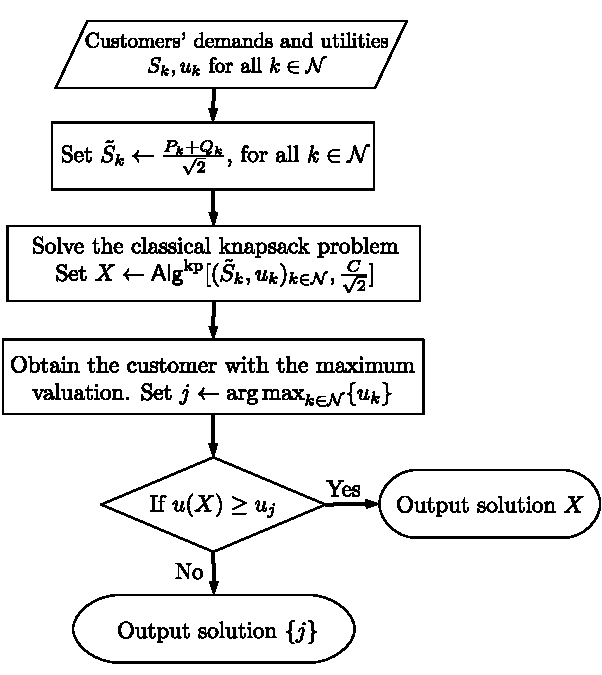
\includegraphics[scale=0.6]{{fig/flow-chart-0.5}.pdf} 
 \caption{Flow chart for One-dimensional Projection Algorithm {\sc (1DPA)}.} %\vspace{-5pt} 
\label{fig:alg0.5}
\end{figure}\vspace{-5pt}


\begin{customthm}{2} \label{thm:1dpa}
Algorithm {\sc 1DPA} produces a feasible solution with a worst-case guarantee $\frac{1}{2}$ with the optimal solution of \textsc{maxPA}.
\end{customthm}
\

Because $\frac{1}{2} \sqrt{\frac{\cos \theta + 1}{2}} \le \frac{1}{2}$, {\sc 1DPA} gives a superior worst-case guarantee than that of {\sc GRA}. The basic idea of the proof is discussed in the Appendix. Algorithm {\sc 1DPA} can be applied to {\sc minPA} by defining the efficiency as ($\frac{c_k}{|S_k|}$). 

Algorithm {\sc 1DPA} can be applied to {\sc minPA} by applying a similar one-dimensional projection approach to reduce the two-dimensional problem into a one-dimensional min-knapsack problem \cite{minKS}.








\iffalse
Now we prove Theorem \ref{thm:2apx}.
\begin{proof}
Let $S^*$ be an optimal solution to C-KP, for which the feasible region is $\cal D$.  Let $S_1^*$, $S_2^*$ be an optimal solution for the subproblem on feasible region ${\cal D}_1$ and ${\cal D}_2$ respectively.  By our observation in Subsection \ref{subsec:pic}, $S_1^*$ is an optimal solution to 1-KP on projected demands and capacity $C/\sqrt{2}$.  Since ${\sc Alg}^{\rm 1d}$ is a $\rho$-approximation algorithm to {\sc 1-KP}, we have $v(S_1)\geq \rho \cdot v(S_1^*)$.  It is also evident that $v(S_2^*)=v(S_2)$.

Next, we analyze the approximation ratio of ${\sc Alg}^{\rm a}$ in three cases.  Here for a subset $S \subseteq K$, we define 
\begin{equation*}
d(S) \triangleq \sum_{k\in S} S_k(t)=\sum_{k\in S} P_k(t)+ {\bf i}\sum_{k\in S} Q_k(t) 
\end{equation*}

\noindent {\bf Case (1): ($\rho$-approximation) } We consider an optimal solution $S^\ast$, such that its sum of demands $d({S^\ast})\in {\cal D}_1$.  

%\begin{proof}
This is an easy case where $v({S^\ast})=v({S_1^\ast})$.  We have $v(S) \ge v(S_1)\ge  \rho \cdot v({S_1^\ast})=\rho \cdot v({S^\ast})$.
%\end{proof}
\vskip 5pt

\noindent {\bf Case (2):  ($\frac{\rho}{1+\rho}$-approximation) } We consider an optimal solution $S^\ast$, such that $d({S^\ast})\in {\cal D}_2$, and there exists an item $j\in S^\ast$ whose demand $d_j\in {\cal D}_2$.  

%\begin{proof}
Let $z \triangleq \sum_{k\in S^\ast\setminus\{j\}} S_k(t)$. Thus, $d({S^\ast})=d_j+z$, i.e., the sum of demands of $S^\ast$ can be written as the sum of a single demand $d_j$ and a subset sum $z$.\footnote{It is possible that $S^{\ast}$ only consists of a single item $j$, in which case our algorithm obviously produces the optimal answer.}  Note that $d_j\in {\cal D}_2$ and $z\in {\cal D}_1$. Otherwise, the projection of $d({S^\ast})=d_j+z$ on the $\frac{\pi}{4}$ line would exceed $2\cdot C/\sqrt{2}>C$.  

Moreover, we have $v({S^\ast\setminus\{j\}}) \le  v({S_1^\ast})$, because $S_1^\ast$ is an optimal solution for feasible region ${\cal D}_1$.  On the other hand, $v_j \le v({S_2})$ since item $j$ with $d_j\in {\cal D}_2$ is a candidate for $S_2$ in our algorithm.  
We obtain:
\begin{equation*}
v({S^\ast})=v_j+v({S^\ast\setminus\{j\}}) \le  v({S_2})+v({S_1^\ast})
\end{equation*}

By the description of our algorithm, the total value of the output solution $v(S)=\max(v({S_1}), v({S_2}))\geq \max(\rho\cdot v({S_1^*}), v({S_2}))= \max(\rho\cdot v({S_1^*}), v({S_2^*}))$.  Now it remains to show that it is further $\geq \frac{\rho}{1+\rho}(v({S_2})+v({S_1^*}))$.

If $\rho\cdot v({S_1^*})\geq v({S_2})$, we have that $v(S)$ is at least 
\begin{equation*}
\rho\cdot v({S_1^*})= \frac{\rho}{1+\rho}(\rho\cdot v({S_1^*})+v({S_1^*}))
\geq \frac{\rho}{1+\rho}( v({S_2})+v({S_1^*}));
\end{equation*}
otherwise, $v(S)$ is at least  
\begin{equation*}
v({S_2})= \frac{\rho}{1+\rho}(v({S_2})+\frac{1}{\rho}v({S_2}))\geq \frac{\rho}{1+\rho}( v({S_2})+v({S_1^*})).
\end{equation*}
%Combining with $\max\{ u(S_1^\ast), u({S_2^\ast})\}\ge \frac{1}{2}\left(u({S_1^\ast})+u({S_2^\ast})\right)$ and $u(S) \ge\rho \cdot \max\{ u(S_1^\ast), u({S_2^\ast})\}$, we get $u(S)\ge \frac{\rho}{2} u({S^\ast})$.

%\end{proof}

\noindent {\bf Case (3): ($\frac{\rho}{2}$-approximation) } We consider an optimal solution $S^\ast$, such that $d({S^\ast})\in {\cal D}_2$, and $S_k(t)\in {\cal D}_1$ for every item $k\in S^\ast$.

%\begin{proof}
First, we let $\tilde{d}(S) \triangleq \sum_{k\in S} \tilde{S}_k$.  The condition on $S^{\ast}$ is equivalent to the following condition on 
projected demands on the $\frac{\pi}{4}$ line: $C/\sqrt{2}<\tilde{d}({S^\ast}) \leq C$, and $\tilde{S}_k \le  C/\sqrt{2}$ for every item $k\in S^\ast$.

We use Lemma \ref{lem:subsetsumA} to show that $d({S^\ast})\in {\cal D}_2$ can be written as the sum of two demand subset sums in ${\cal D}_1$.  Lemma \ref{lem:subsetsumA} is essentially an equivalent statement of this on the projected demands, and will be proved later in this subsection.     

\begin{lemma} \label{lem:subsetsumA}
For a set of $n$ positive real numbers $a_1, ..., a_n$ satisfying $\sum_{i = 1}^n a_i \le C$,  $a_i \le C'$ for all $i$ and $C'\ge C/\sqrt{2}$, there exists a subset $T \subseteq \{1,...,n\}$ such that
\begin{equation*}
\sum_{i \in T} a_i \le C' \mbox{\ \ and \ \ } \sum_{i \in \{1,...,n\} \backslash T} a_i \le C'.
\end{equation*}
\end{lemma}

By Lemma \ref{lem:subsetsumA}, we have $\tilde{d}(T)$ and $\tilde{d}({S^{\ast}\setminus T}) \le  C/\sqrt{2}$ for some subset $T \subseteq S^\ast$. That is, $d(T)  \in {\cal D}_1$ and $d({S^\ast\setminus T}) \in {\cal D}_1$.

Thus, $v(T) \le  v({S_1^\ast})$ and $v({S^\ast\setminus T}) \le  v({S_1^\ast})$.  Moreover, since $v({S^\ast})=v(T)+v({S^\ast\setminus T})$, we have $v({S^\ast}) \le  2v({S_1^\ast})$.  Hence  
\begin{equation*}
v(S) \ge v(S_1)\ge  \rho \cdot v(S_1^\ast)\ge\frac{\rho}{2} v({S^\ast}).
\end{equation*}
%\end{proof}

Combining Cases (1)-(3): $\min\{\rho, \rho/(1+\rho), \rho/2 \} = \rho/2$, we complete the proof of the approximation ratio of ${\sc Alg}^{\rm a}$ as $\rho/2$.
\end{proof}

Finally, we prove Lemma \ref{lem:subsetsumA}:

\begin{proof} 
The case $\sum_{i=1}^{n} a_i\leq C'$ is trivial.  Otherwise, 
let $j$ be the smallest index such that the partial sum exceeds $C'$, i.e., $\sum_{i=1}^{j-1} a_i \le  C'$ and $\sum_{i=1}^{j} a_i>C'$.  Clearly $j \ge 2$ since all $a_i \le  C'$.

Let $x=\sum_{i=1}^{j-1} a_i$, $z=a_j$ and $y = \sum_{i=j+1}^{n} a_i$.  

Note that $\sum_{i = 1}^{n} a_i = x+y+z$.  We already have 
\begin{equation*}
x \le  C',\ \ z \le  C',\ \ 
x+y+z > C' \mbox{\ \ and\ \ } x+z > C'
\end{equation*}

The lemma holds if $y+z \le  C'$, because we can set $T = \{1 ,..., j-1 \}$.  

If $y+z> C'$, then we obtain:
\begin{eqnarray*}
x+y & = & 2(x+y+z)-(x+z)-(y+z)  \\
& < & 2C-2C'\le  (2-\sqrt{2})C  < \frac{C}{\sqrt{2}}\le C'
\end{eqnarray*}
because $x+y+z \le  C$.
Hence, we can set $T = \{1 ,..., j-1, j+1, ..., n\}$.  
\end{proof}
\fi